\documentclass[12pt,UTF8,fleqn]{ctexart}
\usepackage{ctex,amsmath,amssymb,geometry,fancyhdr,bm,amsfonts,mathtools,extarrows,graphicx,url,enumerate,xcolor,float,multicol,wasysym}
\usepackage{subfigure}
\allowdisplaybreaks[4]
% 加入中文支持
\newcommand\Set[2]{\left\{#1\ \middle\vert\ #2 \right\}}
\newcommand\Lim[0]{\lim\limits_{n\rightarrow\infty}}
\newcommand\LIM[2]{\lim\limits_{#1\rightarrow#2}}
\newcommand\Ser[1]{\sum_{n=#1}^\infty}
\newcommand{\SER}[2]{\sum_{#1=#2}^\infty}
\newcommand{\Int}[4]{\varint\nolimits_{#1}^{#2}#3\mathrm d#4}
\newcommand{\aIInt}[1]{\iint\limits_{#1}}
\newcommand{\IInt}[3]{\iint\limits_{#1}#2\mathrm d#3}
\newcommand{\varIInt}[4]{\iint\limits_{#1}#2\mathrm d#3\mathrm d#4}
\newcommand{\IIInt}[3]{\iiint\limits_{#1}#2\mathrm d#3}
\newcommand{\varIIInt}[5]{\iiint\limits_{#1}#2\mathrm d#3\mathrm d#4\mathrm d#5}
\newcommand{\LInt}[3]{\varint\nolimits_{#1}#2\mathrm d#3}
\newcommand{\LOInt}[3]{\varoint\nolimits_{#1}#2\mathrm d#3}
\newcommand{\LLInt}[4]{\varint\nolimits_{#1}\nolimits^{#2}#3\mathrm d#4}
\newcommand{\BLInt}[2]{\varint\nolimits_{#1}#2}
\newcommand{\varBLInt}[3]{\varint\nolimits_{#1}\nolimits^{#2}#3}
\newcommand{\BLOInt}[2]{\varoint\nolimits_{#1}#2}
\newcommand{\SIInt}[3]{\iint\limits_{#1}#2\mathrm d#3}
\newcommand{\md}[1]{\mathrm d#1}
\newcommand{\BSIInt}[2]{\iint\limits_{#1}#2}
\newcommand{\pp}[2]{\frac{\partial #1}{\partial #2}}
\newcommand{\ppx}[1]{\frac{\partial #1}{\partial x}}
\newcommand{\ppy}[1]{\frac{\partial #1}{\partial y}}
\newcommand{\ppz}[1]{\frac{\partial #1}{\partial z}}
\newcommand{\varppx}[1]{\frac{\partial}{\partial x} #1}
\newcommand{\varppy}[1]{\frac{\partial}{\partial y} #1}
\newcommand{\varppz}[1]{\frac{\partial}{\partial z} #1}
\newcommand{\BSOIInt}[2]{\oiint\limits_{#1}#2}
\newcommand{\me}[0]{\mathrm e}
\geometry{a4paper,scale=0.80}
\pagestyle{fancy}
\rhead{向量场的微积分(4)}
\lhead{基础习题课期末复习}
\chead{微积分B(2)}
\begin{document}
\setcounter{section}{12}
\section{专题:格林公式、高斯公式、斯托克斯公式的比较}
\noindent
\subsection{复习计划}
\begin{figure}[H]
\begin{center}
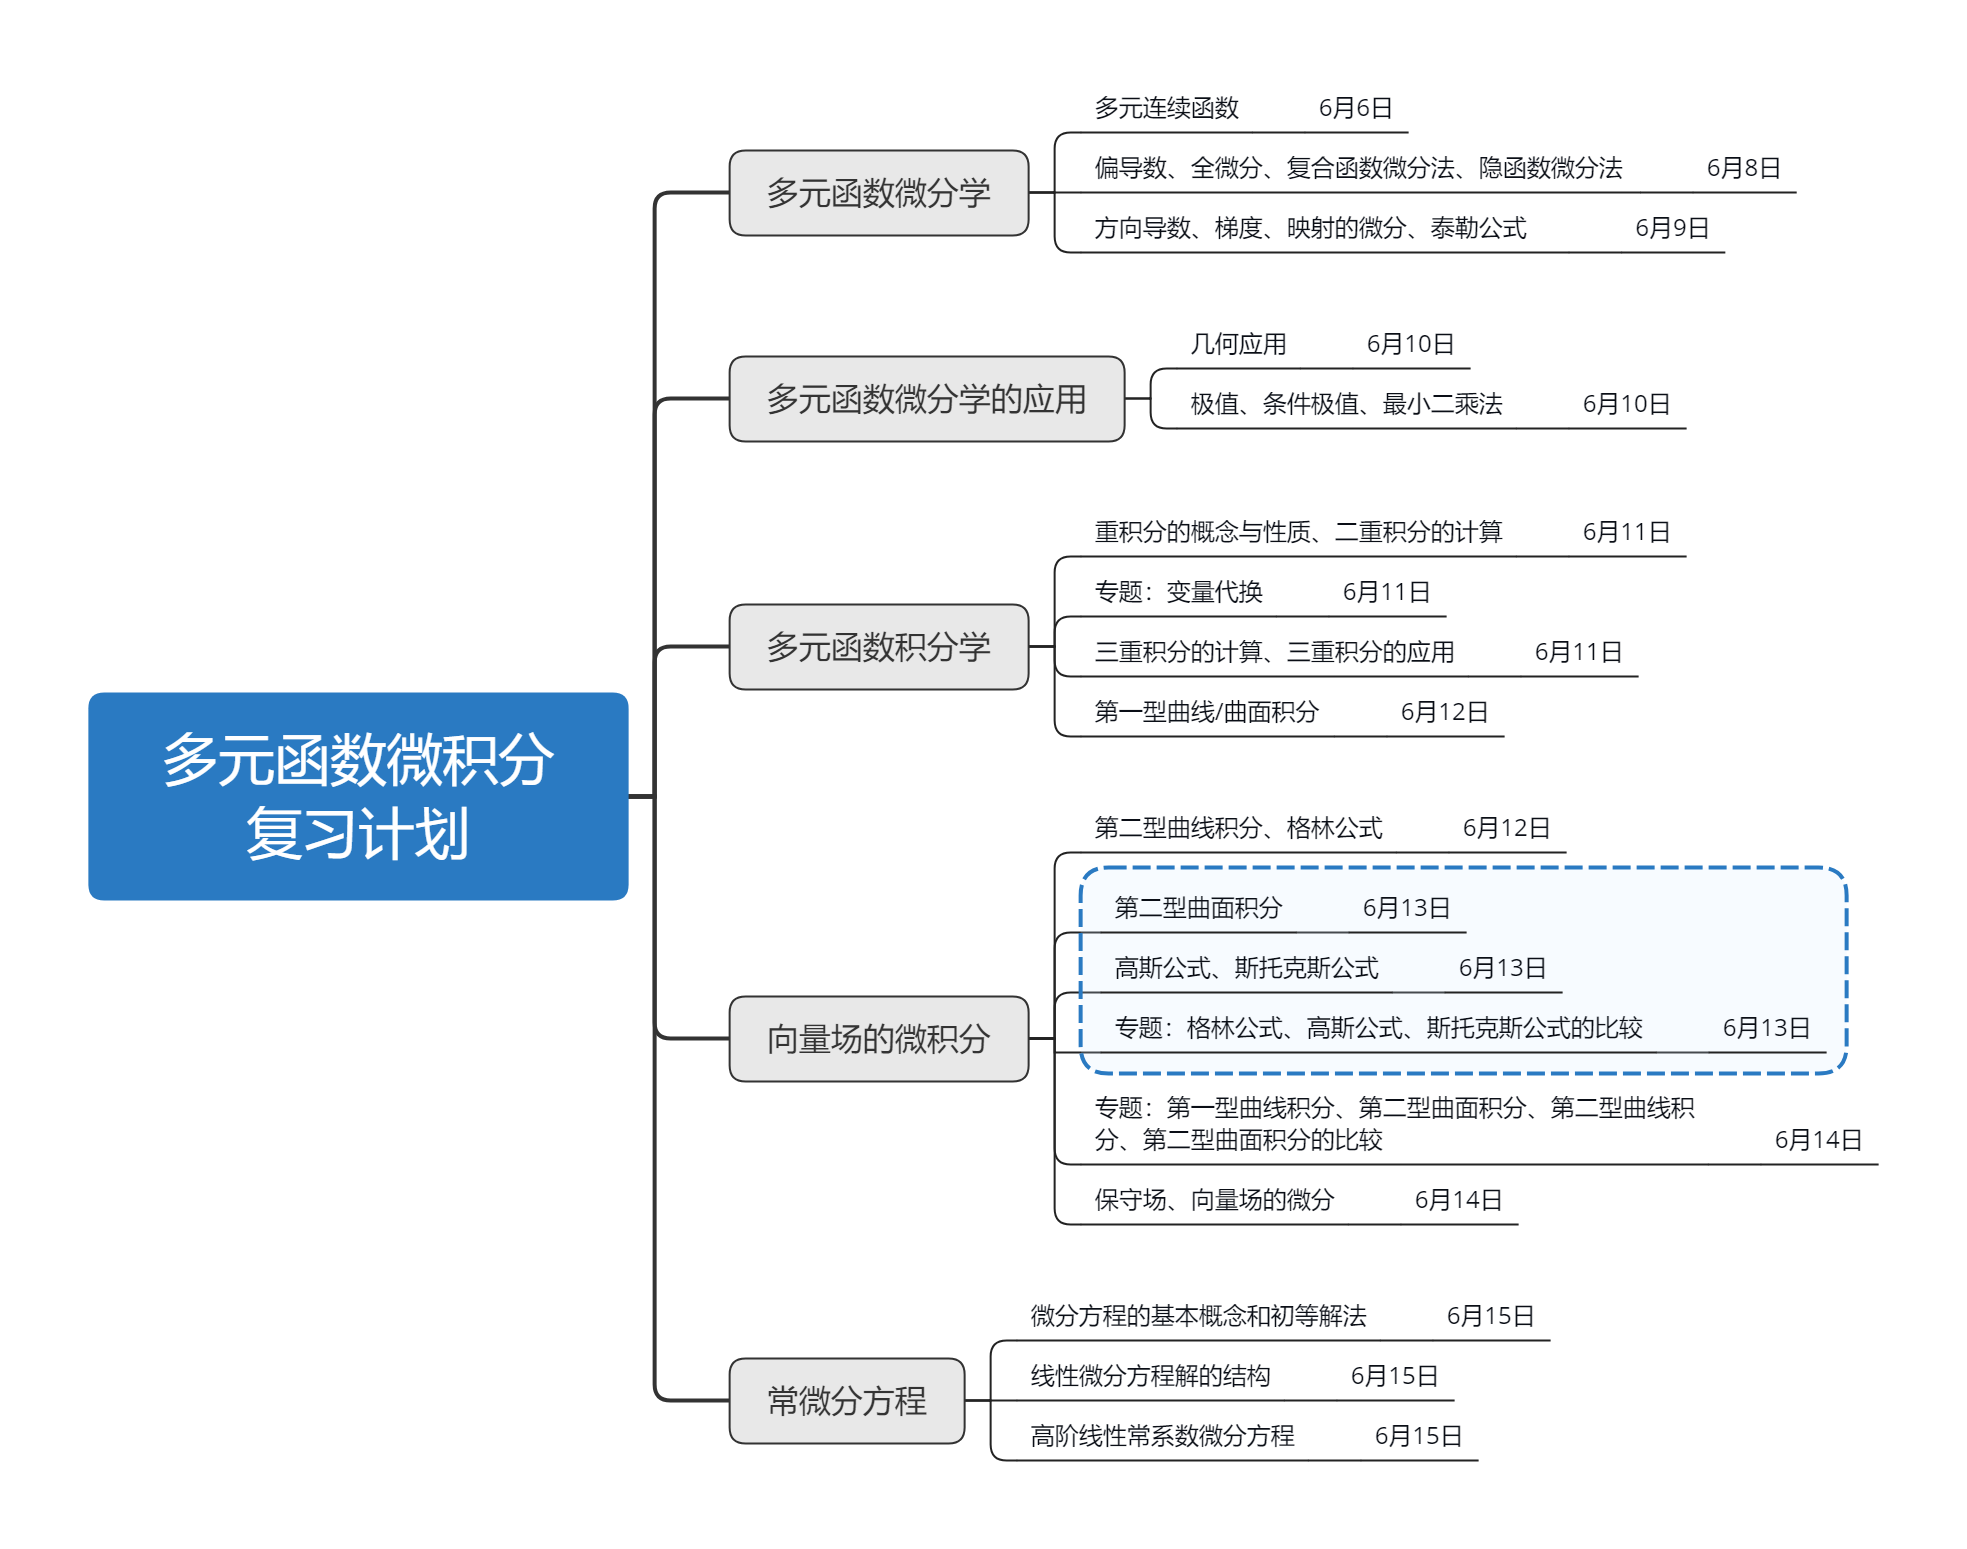
\includegraphics[height=0.5\textheight]{Figures20190613/plan.png}
\end{center}
\end{figure}
\begin{enumerate}
\item[]
\item[]
\item[]
\item[]
\item[]
\item[]
\item[]
\item[]
\end{enumerate}
\subsection{格林公式、高斯公式、斯托克斯公式的图示}
\begin{enumerate}
\item格林公式的图示.
\begin{enumerate}
\item旋度形式(对应于斯托克斯公式在$xOy$平面上的情况):
\begin{figure}[H]
\begin{center}
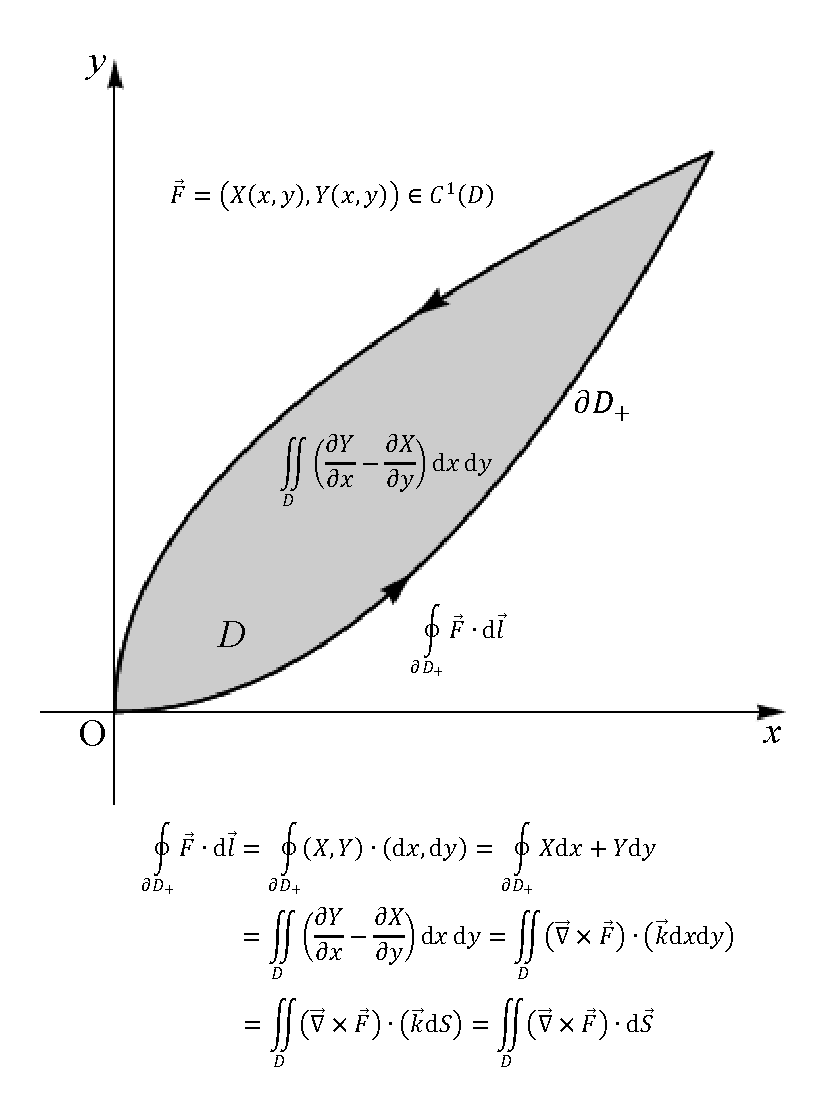
\includegraphics[height=0.618\textheight,angle=0]{Figures20190613/Green.pdf}
\end{center}
\caption{格林公式旋度形式的图示}
\end{figure}
\begin{enumerate}
\item[]
\item[]
\item[]
\item[]
\item[]
\item[]
\end{enumerate}
\item散度形式(对应于高斯公式在$xOy$平面上的情况):
\begin{figure}[H]
\begin{center}
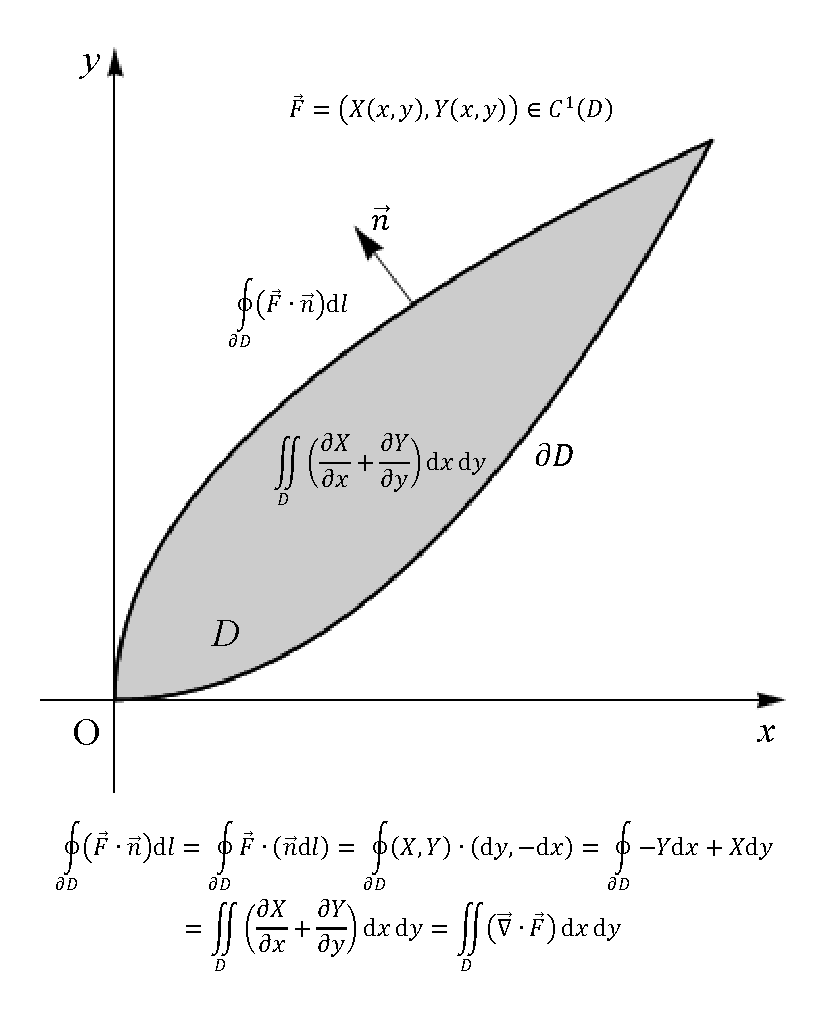
\includegraphics[height=0.618\textheight,angle=0]{Figures20190613/Green2.pdf}
\end{center}
\caption{格林公式散度形式的图示}
\end{figure}
\begin{enumerate}
\item[]
\item[]
\item[]
\item[]
\item[]
\item[]
\item[]
\item[]
\end{enumerate}
\item高斯公式的图示.
\begin{figure}[H]
\begin{center}
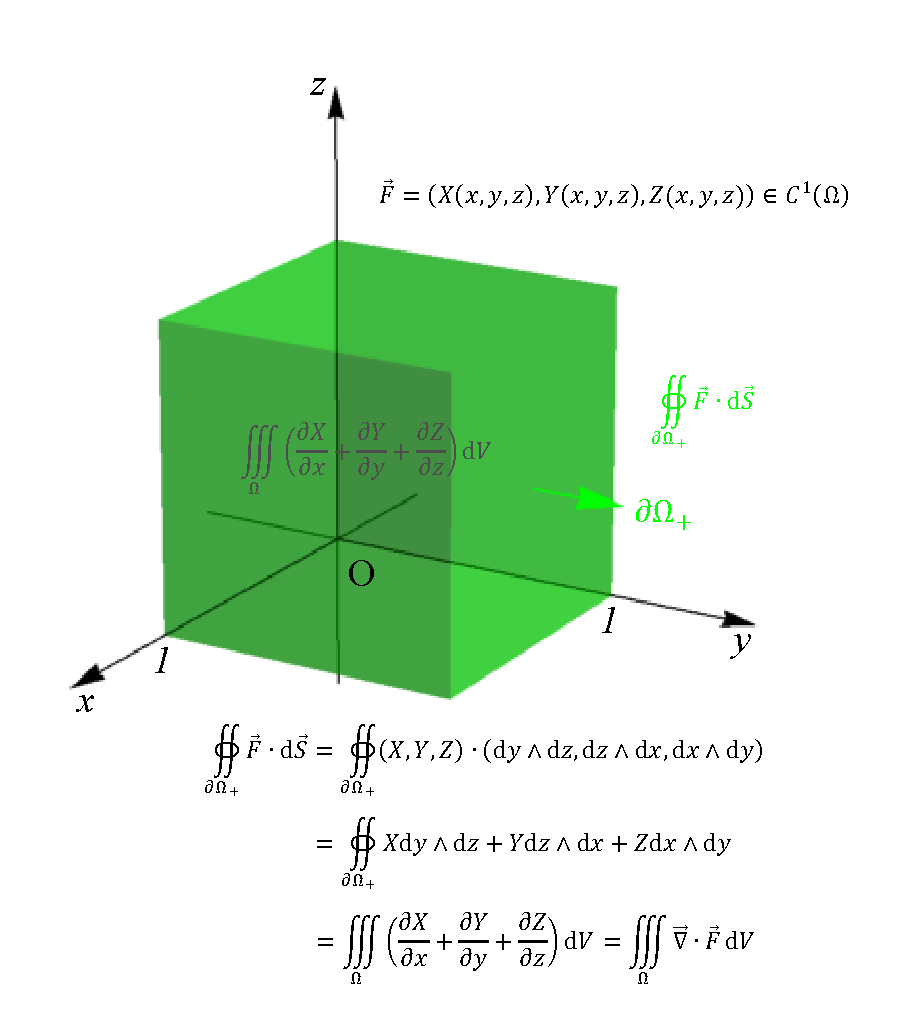
\includegraphics[height=0.618\textheight,angle=0]{Figures20190613/Gauss.pdf}
\end{center}
\caption{高斯公式的图示}
\end{figure}
\end{enumerate}
\begin{enumerate}
\item[]
\item[]
\item[]
\item[]
\item[]
\item[]
\item[]
\item[]
\end{enumerate}
\item斯托克斯公式的图示.
\begin{figure}[H]
\begin{center}
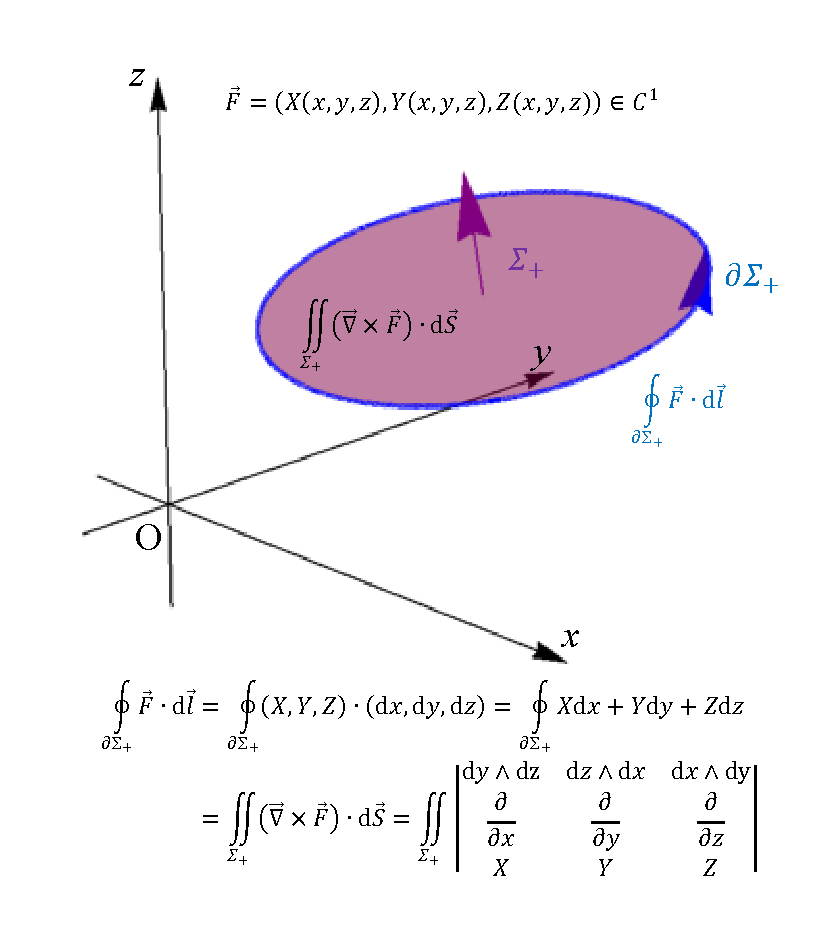
\includegraphics[height=0.618\textheight,angle=0]{Figures20190613/Stokes.pdf}
\end{center}
\caption{斯托克斯公式的图示}
\end{figure}
\end{enumerate}
\subsection{格林公式、高斯公式、斯托克斯公式的比较}
\begin{enumerate}
\item应用场合

\indent格林公式可简化向量场在平面闭合曲线上积分的计算,斯托克斯公式可简化向量场在空间闭合曲线上积分的计算,高斯公式可简化向量场在空间封闭曲面上积分的计算. 可参看后述例题.

对于平面非闭合曲线,可利用积分的线性性质,选取简单曲线补成闭合曲线,以应用格林公式;对于空间非封闭曲面,可利用积分域的可加性,选取简单曲面补成封闭曲面,以应用高斯公式. 可参看后述例题.

应用斯托克斯公式时,应尽量选取空间闭合曲线围成的简单曲面,以使第二型曲面积分的计算尽可能简化. 可参看后述例题.
\item偏导数的连续性(即可微性)

三个公式均要求向量场的各个分量在积分域内有一阶连续偏导数,即可微. 如不满足偏导数连续的条件,可利用积分域的可加性,根据被积函数的形式,选取简单曲线(如圆)或曲面(如球或圆柱面),将偏导数不连续的点去掉. 可参看后述例题.

%格林公式要求向量场的各个分量在闭合曲线围成的区域内有一阶连续的偏导数,即可微. 如不满足偏导数连续的条件,可根据被积函数的形式,选取简单曲线(如圆)将偏导数不连续的点去掉. 可参看后述例题.
%
%高斯公式要求向量场的各个分量在封闭曲面围成的空间区域内有一阶连续的偏导数,即可微. 如不满足偏导数连续的条件,可根据被积函数的形式,选取简单曲面(如球)将偏导数不连续的点去掉. 可参看后述例题.
%
%斯托克斯公式要求向量场的各个分量在曲线和曲面所在的区域内有一阶连续的偏导数,即可微. 如不满足偏导数连续的条件,可根据被积函数的形式,选取简单曲面,将偏导数不连续的点去掉. 可参看后述例题.
\item方向性

根据右手法则,格林公式应用于单连通域时,边界曲线逆时针为正;应用于复连通域时,外边界逆时针为正向,内边界顺时针为正向.

斯托克斯公式中曲线的方向和曲面方向之间应符合右手法则;对于复连通曲面,曲面外边界线和内边界线的方向相反,不必规定边界曲线的顺时针或逆时针方向.

高斯公式应用于空间单连通域时,边界曲面的外侧为正;应用于空间复连通域时,外边界曲面外侧为正,内边界曲面内侧为正.


\item空间公式向平面公式的转化

格林公式用于计算平面闭合曲线的第二型曲线积分,斯托克斯公式用于计算空间闭合曲线的第二型曲线积分. 将斯托克斯公式应用于$xOy$平面上的闭合曲线,得到的公式形式与格林公式相同.

格林公式的散度形式将向量场在平面闭合曲线的外向通量与向量场的散度在该曲线围成的平面区域内的二重积分联系起来,高斯公式将向量场在空间闭合曲面的外向通量与向量场的散度在该曲面围成的空间区域上的三重积分联系起来. 将高斯公式中的封闭曲面换成曲线,曲面积分换成曲线积分,空间域换成平面域,三重积分换成二重积分,可将高斯公式化成格林公式.

斯托克斯公式化成格林公式的旋度形式,与高斯公式化成格林公式的散度形式,两种转化方式有所区别. 
\end{enumerate}
\subsection{主要题型}
\begin{enumerate}
\item直接应用格林公式、高斯公式和斯托克斯公式求解.

【具体使用方法可见例1、例2、例3.】
\item对于非封闭曲线或非封闭曲面,利用积分域的可加性,选取简单曲线或曲面构造封闭曲线或曲面,以应用格林公式和高斯公式. 

【具体使用方法可见例4.】
\item格林公式、高斯公式和斯托克斯公式均要求函数在积分域内有一阶连续偏导数,如在积分域内存在一阶连续偏导数不连续的点(奇异点),可利用积分域的可加性,选取简单曲线或曲面,将奇异点去除,从而应用格林公式、高斯公式或斯托克斯公式求解.  

【具体使用方法可见例5、例6、例7.】
\item利用格林公式的散度形式进行证明.

【具体使用方法可见例8.】
\item应用斯托克斯公式时应选取简单的曲面(如平面),使曲面积分的求解尽量简单.

【如例9.】
\item应用题:应用高斯公式证明电场的高斯定理.

【如例10.】
\end{enumerate}
\subsection{例题}
\begin{enumerate}
\item[例1]$\BLOInt L{(x^2+y^2)\md x+(y^2-x^2)\md y}$,其中$L$是区域$D$的边界正向(逆时针),区域$D$由直线$y=0,x=1,y=x$围成.

\begin{figure}[H]
\begin{center}
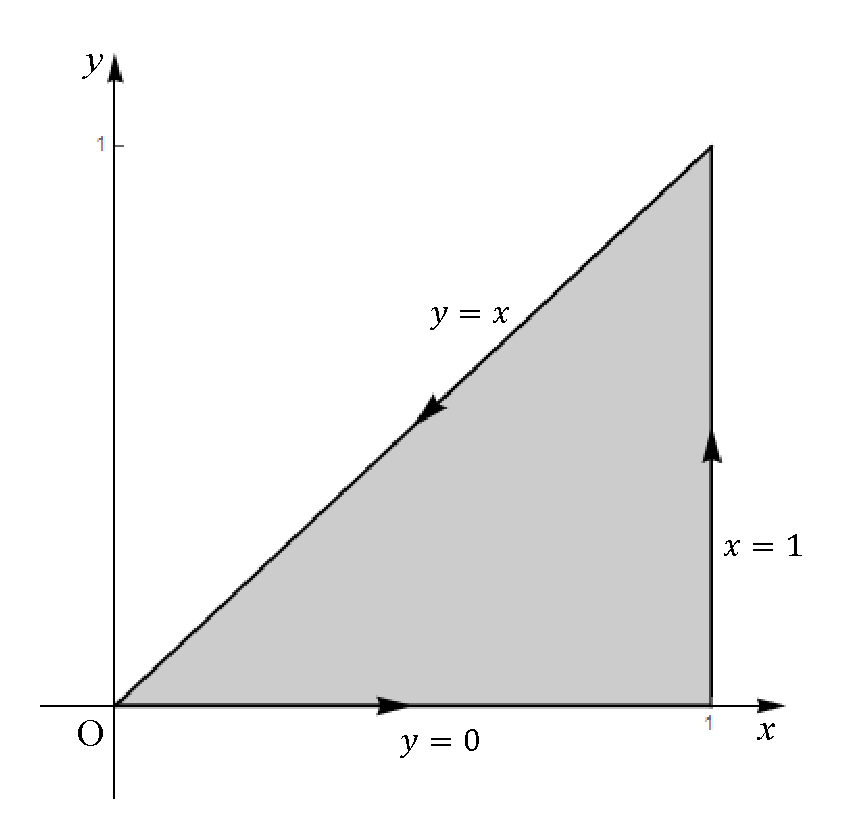
\includegraphics[height=0.3\textheight]{Figures20190613/Fig13-3-1-3.pdf}
\end{center}
\caption{例1图示}
\label{13-3-1-3}
\end{figure}

解:$\because\frac{\partial(y^2-x^2)}{\partial x}=-2x,\ \frac{\partial(x^2+y^2)}{\partial y}=2y$均在$D$上连续,

$\therefore\BLOInt L{(x^2+y^2)\md x+(y^2-x^2)\md y}=\varIInt D{[\frac{\partial(y^2-x^2)}{\partial x}-\frac{\partial(x^2+y^2)}{\partial y}]}xy=\varIInt D{(-2x-2y)}xy\\
=\Int01{}x\Int0x{(-2x-2y)}y=\Int01{(-2xy-y^2)\big|_0^x}x=\Int01{-2x^2-x^2}x=-x^3\big|_0^1=-1$.
\item[例2]$\BSIInt S{x^2\md y\wedge\md z+y^2\md z\wedge\md x+z^2\md x\wedge\md y}$,其中$S$为正方体$\Omega:\ 0\leqslant x\leqslant1,0\leqslant y\leqslant1,0\leqslant z\leqslant1$的外表面.

\begin{figure}[H]
\begin{center}
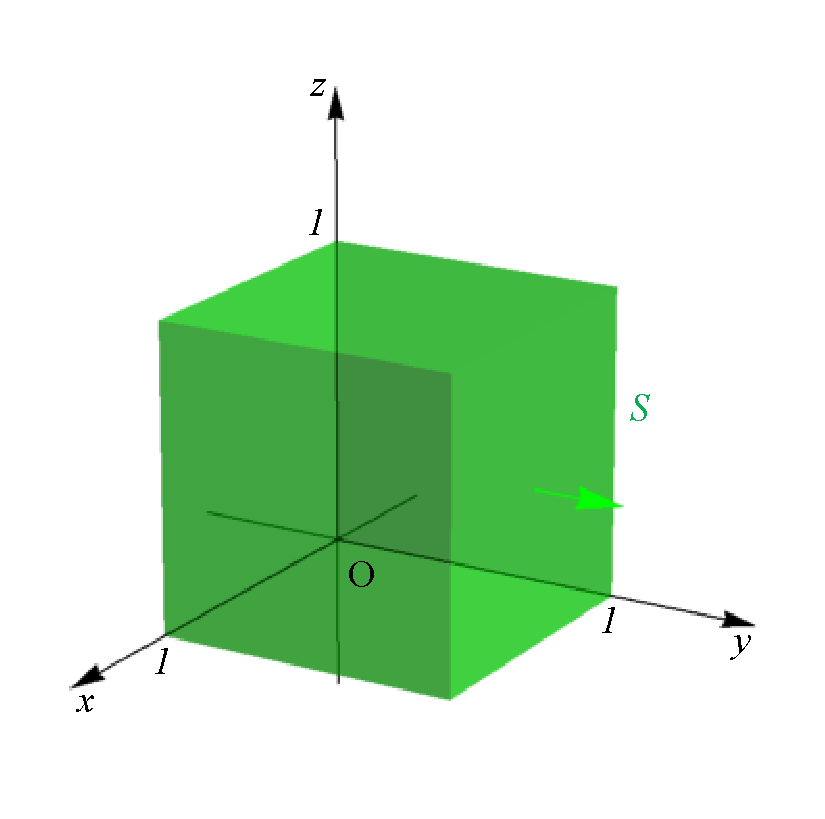
\includegraphics[height=0.5\textheight]{Figures20190613/Fig13-5-1-3.pdf}
\end{center}
\caption{例2图示}
\label{13-5-1-3}
\end{figure}

解:$\because x^2,y^2,z^2\in C^1(\Omega)$,

$\therefore\BSIInt S{x^2\md y\wedge\md z+y^2\md z\wedge\md x+z^2\md x\wedge\md y}=\varIIInt\Omega{(\pp{x^2}x+\pp{y^2}y+\pp{z^2}z)}xyz\\
=2\varIIInt\Omega{(x+y+z)}xyz=6\varIIInt\Omega xxyz=6\Int01xx\Int01{}y\Int01{}z=6\Int01xx\Int01{}y\\
=6\Int01xx=3x^2\big|_0^1=3$.

\item[例3]$\BLOInt L{(y-x)\md x+(z-y)\md y+(x-z)\md z}$,其中$L$是柱面$x^2+y^2=a^2$与平面$x+z=a(a>0)$的交线,从$x$轴正向看去为逆时针方向.

\begin{figure}[H]
\begin{center}
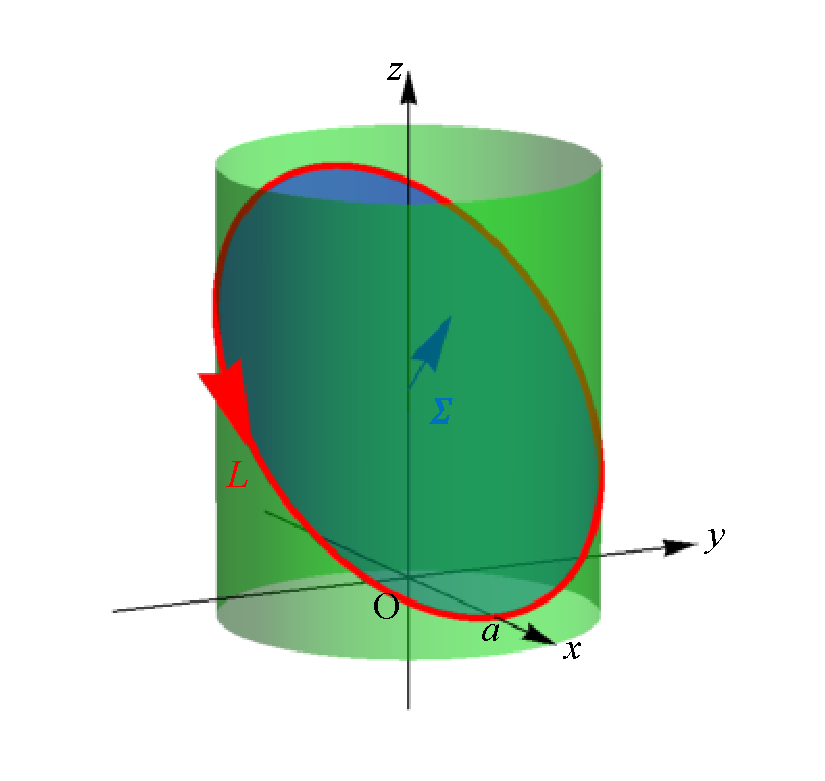
\includegraphics[height=0.5\textheight]{Figures24/Fig13-5-2-2.pdf}
\end{center}
\caption{例3图示}
\label{13-5-2-2}
\end{figure}

解:记$\Sigma$是平面$x+z=a$上$L$围成的部分,$\Sigma$的方向与$L$的方向符合右手法则,即$\Sigma$的上侧为正,

$\because y-x,z-y,x-z\in C^1$,

$\therefore\BLOInt L{(y-x)\md x+(z-y)\md y+(x-z)\md z}=\BSIInt\Sigma{\begin{vmatrix}
\bm i&\bm j&\bm k\\
\frac\partial{\partial x}&\frac\partial{\partial y}&\frac\partial{\partial z}\\
y-x&z-y&x-z
\end{vmatrix}\bm\cdot\md\bm S}\\
=\BSIInt\Sigma{(\pp{(x-z)}y-\pp{(z-y)}z,\pp{(y-x)}z-\pp{(x-z)}x,\pp{(z-y)}x-\pp{(y-x)}y)\bm\cdot\md\bm S}=\BSIInt\Sigma{(0-1,0-1,0-1)\bm\cdot\md\bm S}$,

$\because$在$\Sigma:z=a-x,x^2+y^2\leqslant a^2$的上侧\\
$\md\bm S=(-\pp zx,-\pp zy,1)\md x\md y=(1,0,1)\md x\md y=(\md y\wedge\md z,\md z\wedge\md x,\md x\wedge\md y)$,

$\therefore$上式$=\varIInt{x^2+y^2\leqslant a^2}{(0-1,0-1,0-1)\bm\cdot(1,0,1)}xy=-2\varIInt{x^2+y^2\leqslant a^2}{}xy=-2\pi a^2$.
\item[例4]$\BSIInt S{x^2\md y\wedge\md z+(z^2-2z)\md x\wedge\md y}$,其中$S$为$z=\sqrt{x^2+y^2}$被平面$z=0$和$z=1$所截部分的外侧.

\begin{figure}[H]
\begin{center}
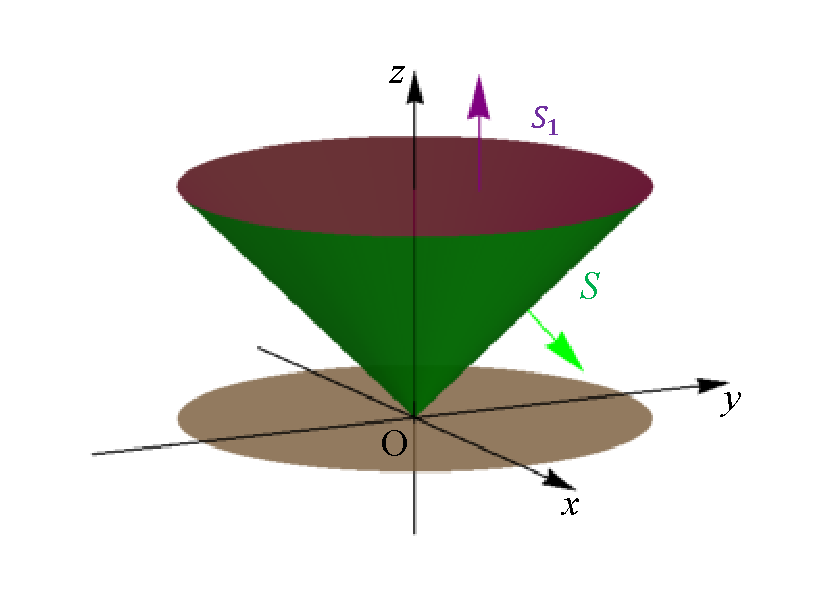
\includegraphics[height=0.5\textheight]{Figures24/Fig13-5-1-5.pdf}
\end{center}
\caption{例4图示}
\label{13-5-1-5}
\end{figure}

解:取平面$S_1:z=1,x^2+y^2\leqslant1$,上侧为正,记$S$与$S_1$围成的区域为$\Omega$,

$\because x^2,z^2-2z\in C^1(\Omega)$,

$\therefore\BSIInt{S+S_1}{x^2\md y\wedge\md z+(z^2-2z)\md x\wedge\md y}=\varIIInt\Omega{(\pp{x^2}x+\pp0y+\pp{(z^2-2z)}z)}xyz\\
=\varIIInt\Omega{(2x+2z-2)}xyz$,

由对称性可知$\varIIInt\Omega{2x}xyz=0$,

$\therefore$上式$=\varIIInt\Omega{(2z-2)}xyz=\Int01{(2z-2)}z\varIInt{x^2+y^2\leqslant z^2}{}xy=\Int01{(2z-2)\pi z^2}z\\
=2\pi\Int01{(z^3-z^2)}z=2\pi(\frac14z^4-\frac13z^3)\big|_0^1=-\frac16\pi$,

$\because$在$S_1$上$\md\bm S=(-\pp zx,-\pp zy,1)\md x\md y=(0,0,1)\md x\md y=(\md y\wedge\md z,\md z\wedge\md x,\md x\wedge\md y)$,

$\therefore\BSIInt{S_1}{x^2\md y\wedge\md z+(z^2-2z)\md x\wedge\md y}=\varIInt{x^2+y^2\leqslant1}{[x^2\cdot0+(1^2-2\cdot1)]}xy=-\varIInt{x^2+y^2\leqslant1}{}xy=-\pi$,

$\therefore\BSIInt S{x^2\md y\wedge\md z+(z^2-2z)\md x\wedge\md y}=-\frac\pi6-\BSIInt{S_1}{x^2\md y\wedge\md z+(z^2-2z)\md x\wedge\md y}=-\frac\pi6+\pi=\frac56\pi$.
\item[例5]计算$I=\BLOInt L{\frac{(x+y)\mathrm dx-(x-y)\mathrm dy}{x^2+y^2}}$,其中$L$:\\
(1)$D=\Set{(x,y)}{r^2\leqslant x^2+y^2\leqslant R^2}(0<r<R)$;\\
(2)$D=\Set{(x,y)}{\frac{x^2}{a^2}+\frac{y^2}{b^2}}$的正向边界.

\begin{figure}[H]
\begin{center}
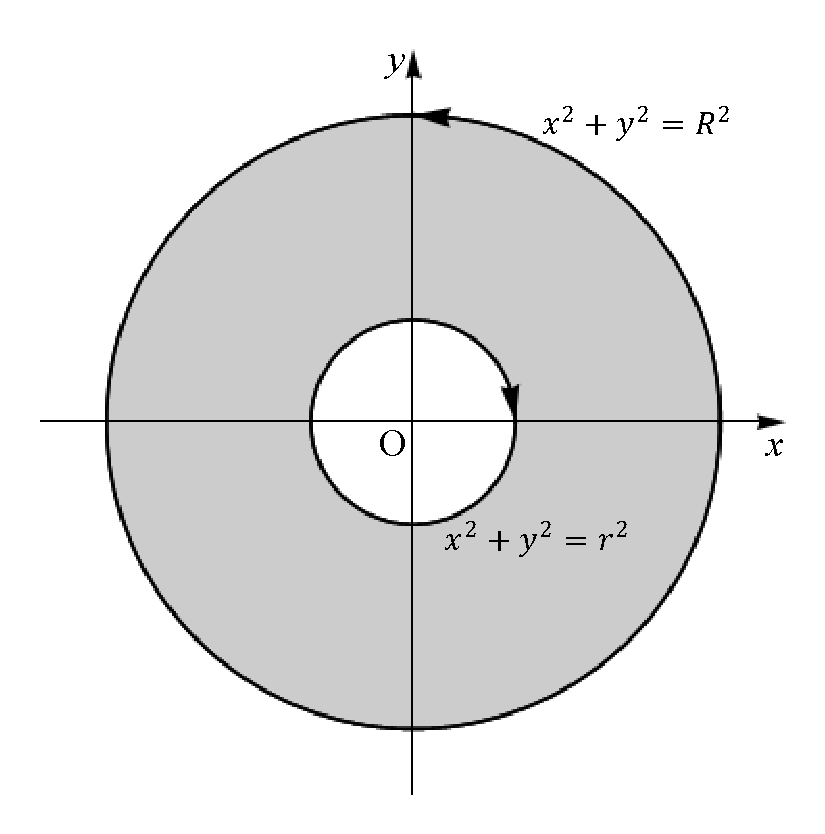
\includegraphics[height=0.3\textheight]{Figures20190613/Fig13-3-2-1.pdf}
\end{center}
\caption{例5(1)题图示}
\label{13-3-2-1}
\end{figure}


解:令$Y(x,y)=-\frac{x-y}{x^2+y^2},X(x,y)=\frac{x+y}{x^2+y^2}$,则\[\begin{split}
\frac{\partial Y(x,y)}{\partial x}&=\frac{-(x^2+y^2)+(x-y)\cdot2x}{(x^2+y^2)^2}=\frac{x^2-y^2-2xy}{(x^2+y^2)^2},\\
\frac{\partial X(x,y)}{\partial y}&=\frac{x^2+y^2-(x+y)\cdot2y}{(x^2+y^2)^2}=\frac{x^2-y^2-2xy}{(x^2+y^2)^2}.
\end{split}\]

(1)$\because\frac{\partial Y(x,y)}{\partial x},\frac{\partial X(x,y)}{\partial y}$在$D=\Set{(x,y)}{r^2\leqslant x^2+y^2\leqslant R^2}(0<r<R)$上连续,

$\therefore$
\[I=\varIInt D{[\frac{\partial Y(x,y)}{\partial x}-\frac{\partial X(x,y)}{\partial y}]}xy=0.\]

\begin{figure}[H]
\begin{center}
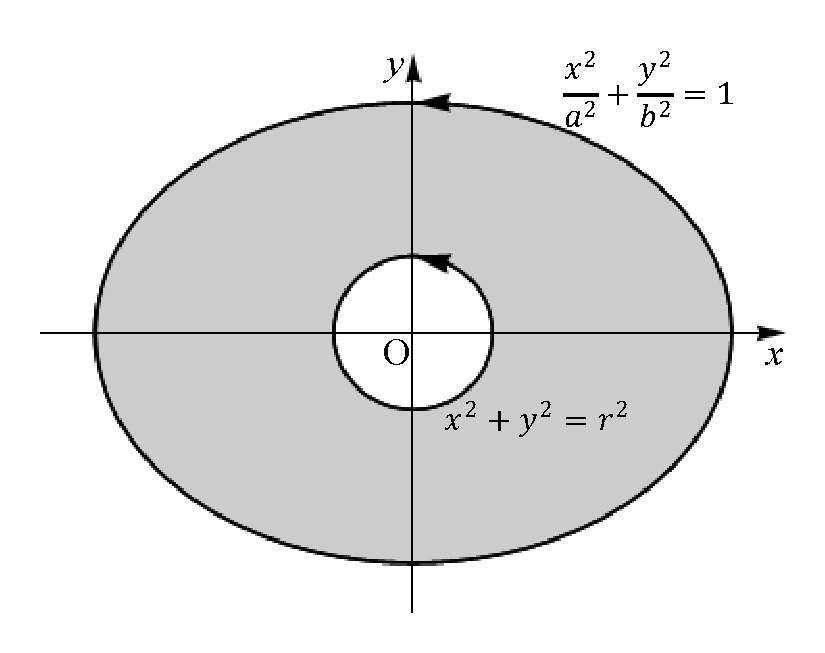
\includegraphics[height=0.3\textheight]{Figures20190613/Fig13-3-2-2.pdf}
\end{center}
\caption{例5(2)题图示}
\label{13-3-2-2}
\end{figure}

(2)取正向圆周$L_1:x^2+y^2=r^2,r<\min\{a,b\}$,记其围成的区域为$D_1$,则$\frac{\partial Y(x,y)}{\partial x},\frac{\partial X(x,y)}{\partial y}$\\
在$L$和$L_{1-}$围成的区域$D^*$内连续,

$\therefore$
\[\BLOInt{L+L_{1-}}{\frac{(x+y)\mathrm dx-(x-y)\mathrm dy}{x^2+y^2}}=\varIInt{D^*}{[\frac{\partial Y(x,y)}{\partial x}-\frac{\partial X(x,y)}{\partial y}]}xy=0,\]

$\therefore$
\[(\varoint\nolimits_L+\BLOInt{L_{1-}}{)\frac{(x+y)\mathrm dx-(x-y)\mathrm dy}{x^2+y^2}}=I+\BLOInt{L_{1-}}{\frac{(x+y)\mathrm dx-(x-y)\mathrm dy}{x^2+y^2}}=0,\]

$\therefore$
\[\begin{split}
I&=-\BLOInt{L_{1-}}{\frac{(x+y)\mathrm dx-(x-y)\mathrm dy}{x^2+y^2}}=\BLOInt{L_{1+}}{\frac{(x+y)\mathrm dx-(x-y)\mathrm dy}{x^2+y^2}}\\
&=\frac1{r^2}\BLOInt{L_{1+}}{(x+y)\mathrm dx-(x-y)\mathrm dy}\\
&=\frac1{r^2}\varIInt{D_1}{[\frac{\partial(-x+y)}{\partial x}-\frac{\partial(x+y)}{\partial y}]}xy\\
&=\frac1{r^2}\varIInt{D_1}{-2}xy=\frac1{r^2}(-2)\pi r^2=-2\pi.
\end{split}\]
\item[例6]$\BSOIInt S{\frac{x\md y\wedge\md z+y\md z\wedge\md x+z\md x\wedge\md y}{(x^2+y^2+z^2)^{\frac32}}}$,其中$S$为椭球面$\frac{x^2}{a^2}+\frac{y^2}{b^2}+\frac{z^2}{c^2}=1$.

\begin{figure}[H]
\begin{center}
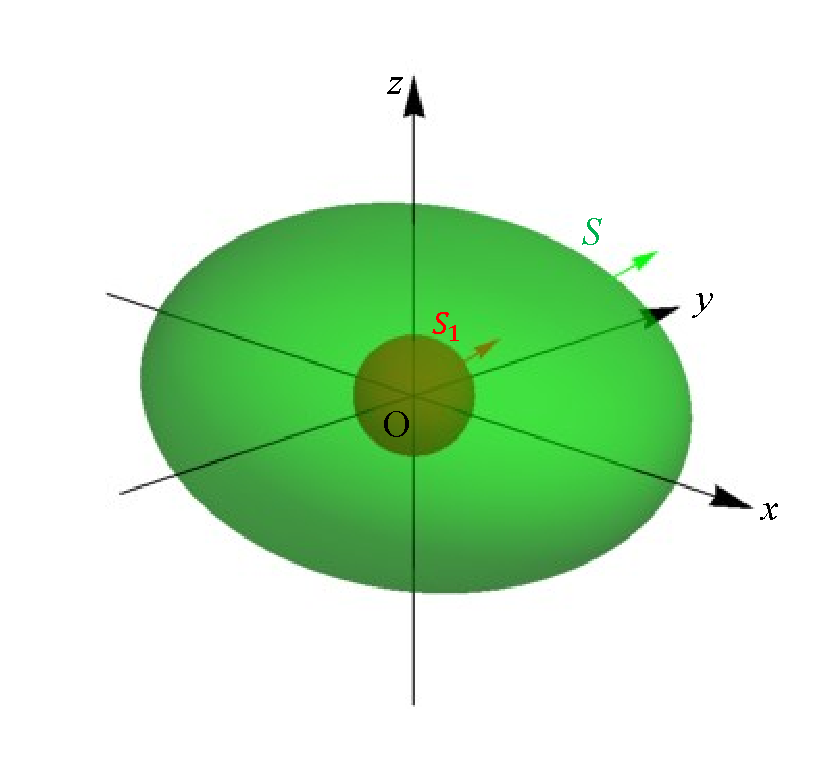
\includegraphics[height=0.5\textheight]{Figures24/Fig13-5-1-7.pdf}
\end{center}
\caption{例6图示}
\label{13-5-1-7}
\end{figure}

解:取球面$S_1:\ x^2+y^2+z^2=r^2,r<\min\{a,b,c\}$,外侧为正,设$S$与$S_1^-$围成的区域为$\Omega$,$S_1$围成的区域为$\Omega_1$,

则$X=\frac x{(x^2+y^2+z^2)^{\frac32}},\ Y=\frac y{(x^2+y^2+z^2)^{\frac32}},\ Z=\frac z{(x^2+y^2+z^2)^{\frac32}}\in C^1(\Omega)$,
\[\begin{aligned}
\pp Xx=\frac{(x^2+y^2+z^2)^{\frac32}-x\cdot\frac32(x^2+y^2+z^2)^{\frac12}\cdot2x}{(x^2+y^2+z^2)^3}=\frac{y^2+z^2-2x^2}{(x^2+y^2+z^2)^{\frac52}},\\
\pp Yy=\frac{(x^2+y^2+z^2)^{\frac32}-y\cdot\frac32(x^2+y^2+z^2)^{\frac12}\cdot2y}{(x^2+y^2+z^2)^3}=\frac{z^2+x^2-2y^2}{(x^2+y^2+z^2)^{\frac52}},\\
\pp Zz=\frac{(x^2+y^2+z^2)^{\frac32}-z\cdot\frac32(x^2+y^2+z^2)^{\frac12}\cdot2z}{(x^2+y^2+z^2)^3}=\frac{x^2+y^2-2z^2}{(x^2+y^2+z^2)^{\frac52}},
\end{aligned}\]

$\therefore$
\[\begin{aligned}
&\BSOIInt{S+S_1^-}{\pp Xx\md y\wedge\md z+\pp Yy\md z\wedge\md x+\pp Zz\md x\wedge\md y}=\varIIInt\Omega{(\pp Xx+\pp Yy+\pp Zz)}xyz\\
=&\varIIInt\Omega{\frac{y^2+z^2-2x^2+z^2+x^2-2y^2+x^2+y^2-2z^2}{(x^2+y^2+z^2)^{\frac52}}}xyz=\varIIInt\Omega{0}xyz=0,
\end{aligned}\]
$\therefore$
\[\begin{aligned}
&\BSOIInt S{\frac{x\md y\wedge\md z+y\md z\wedge\md x+z\md x\wedge\md y}{(x^2+y^2+z^2)^{\frac32}}}=0-\BSOIInt{S_1^-}{\frac{x\md y\wedge\md z+y\md z\wedge\md x+z\md x\wedge\md y}{(x^2+y^2+z^2)^{\frac32}}}\\
=&\BSOIInt{S_1}{\frac{x\md y\wedge\md z+y\md z\wedge\md x+z\md x\wedge\md y}{(x^2+y^2+z^2)^{\frac32}}}=\BSOIInt{S_1}{\frac{x\md y\wedge\md z+y\md z\wedge\md x+z\md x\wedge\md y}{(r^2)^{\frac32}}}\\=&\frac1{r^3}\BSOIInt{S_1}{x\md y\wedge\md z+y\md z\wedge\md x+z\md x\wedge\md y}=\frac1{r^3}\varIIInt\Omega{(\pp xx+\pp yy+\pp zz)}xyz\\
=&\frac3{r^3}\varIIInt\Omega{}xyz=\frac3{r^3}\frac43\pi r^3=4\pi.
\end{aligned}\]

\item[例7]计算$I=\BLOInt L{\frac{-y\md x+x\md y}{x^2+y^2}+z\md z}$,其中$L$是:\\
(1)任意一条既不环绕$z$轴,也不与$z$轴相交的简单闭曲线;\\
(2)任意一条环绕$z$轴一圈且不与$z$轴相交的简单闭曲线,从$z$轴正向看去为逆时针方向.

\begin{figure}[H]
\begin{center}
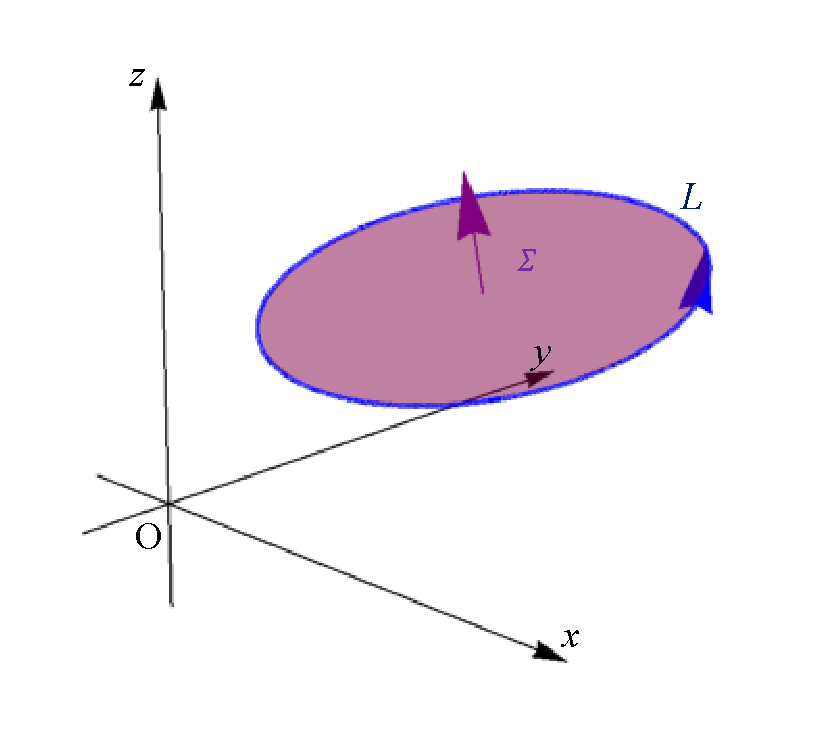
\includegraphics[height=0.5\textheight]{Figures24/Fig13-5-3-1.pdf}
\end{center}
\caption{例7(1)题图示}
\label{13-5-3-1}
\end{figure}

解:(1)取曲面$\Sigma$为曲线$L$围成的逐片光滑有向曲面,$\Sigma$和$L$的方向符合右手法则,$z$轴不穿过$\Sigma$,

则$X=\frac{-y}{x^2+y^2},\ Y=\frac x{x^2+y^2},\ Z=z\in C^1$,

$\therefore$
\[\begin{aligned}
I&=\BLOInt L{X\md x+Y\md y+Z\md z}=\BSIInt\Sigma{\begin{vmatrix}
\bm i&\bm j&\bm k\\
\frac\partial{\partial x}&\frac\partial{\partial y}&\frac\partial{\partial z}\\
X&Y&Z
\end{vmatrix}}\bm\cdot\md\bm S=\BSIInt\Sigma{\begin{vmatrix}
\bm i&\bm j&\bm k\\
\frac\partial{\partial x}&\frac\partial{\partial y}&\frac\partial{\partial z}\\
\frac{-y}{x^2+y^2}&\frac x{x^2+y^2}&z
\end{vmatrix}}\bm\cdot\md\bm S\\
&=\BSIInt\Sigma{(\frac{\partial z}{\partial y}-\frac\partial{\partial z}\frac x{x^2+y^2},\frac\partial{\partial z}\frac{-y}{x^2+y^2}-\frac{\partial z}{\partial x},\frac\partial{\partial x}\frac x{x^2+y^2}-\frac\partial{\partial y}\frac{-y}{x^2+y^2})\bm\cdot\md\bm S}\\
&=\BSIInt\Sigma{(0-0,0-0,\frac{(x^2+y^2)-x\cdot2x}{(x^2+y^2)^2}-\frac{-(x^2+y^2)+y\cdot2y}{(x^2+y^2)^2})\bm\cdot\md\bm S}\\
&=\BSIInt\Sigma{(0,0,0)\bm\cdot\md\bm S}=0.
\end{aligned}\]

\begin{figure}[H]
\begin{center}
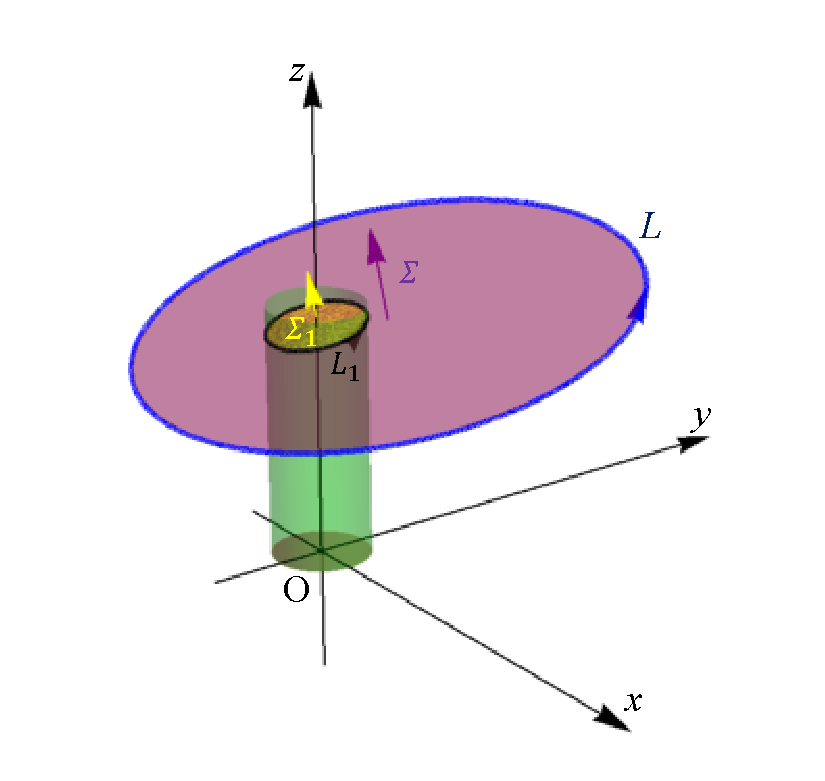
\includegraphics[height=0.7\textheight]{Figures24/Fig13-5-3-2.pdf}
\end{center}
\caption{例7(2)题图示}
\label{13-5-3-2}
\end{figure}

(2)设曲面$\Sigma$为曲线$L$围成的逐片光滑有向曲面,$\Sigma$与$L$的方向符合右手法则,即$\Sigma$的上侧为正,此时$z$轴穿过$\Sigma$. 取柱面$x^2+y^2=r^2$与$\Sigma$交于曲线$L_1$,$r$应足够小使得闭合交线$L_1$全部位于$\Sigma$上,设从$z$轴正向看去$L_1$为逆时针方向. 记$\Sigma_1$为$L_1$围成的逐片光滑正向曲面,$\Sigma_2$为$L$与$L_1^-$围成的逐片光滑正向曲面, $\Omega_2=\mathbb R^3\backslash\{(x,y)|x^2+y^2<r^2\}$.

则$X=\frac{-y}{x^2+y^2},\ Y=\frac x{x^2+y^2},\ Z=z\in C^1(\Omega_2)$,

与(1)同理可知$\BLOInt{L+L_1^-}{X\md x+Y\md y+Z\md z}=0$,

$\therefore$
\[\begin{aligned}
I&=0-\BLOInt{L_1^-}{X\md x+Y\md y+Z\md z}=\BLOInt{L_1}{X\md x+Y\md y+Z\md z}\\
&=\BLOInt{L_1}{\frac{-y\md x+x\md y}{x^2+y^2}+z\md z}=\BLOInt{L_1}{\frac{-y\md x+x\md y}{r^2}+z\md z}\\
&=\BSIInt{\Sigma_1}{\begin{vmatrix}
\bm i&\bm j&\bm k\\
\frac\partial{\partial x}&\frac\partial{\partial y}&\frac\partial{\partial z}\\
-\frac y{r^2}&\frac x{r^2}&z
\end{vmatrix}\bm\cdot\md\bm S}=\BSIInt{\Sigma_1}{(\pp zy-\frac\partial{\partial z}\frac x{r^2},\frac\partial{\partial z}(-\frac y{r^2})-\pp zx,\frac\partial{\partial x}\frac x{r^2}-\frac\partial{\partial y}(-\frac y{r^2}))\bm\cdot\md\bm S}\\
&=\BSIInt{\Sigma_1}{(0-0,0-0,\frac 1{r^2}-(-\frac 1{r^2}))\bm\cdot\md\bm S}=\BSIInt{\Sigma_1}{(0,0,\frac 2{r^2})\bm\cdot(\md y\wedge\md z,\md z\wedge\md x,\md x\wedge\md y)}\\
&=\BSIInt{\Sigma_1}{\frac 2{r^2}\md x\wedge\md y}=\frac 2{r^2}\BSIInt{\Sigma_1}{\md x\wedge\md y},
\end{aligned}\]
$\because\Sigma_1$方程可表示为$z=f(x,y),x^2+y^2\leqslant r^2$,且$\Sigma_1$上侧为正,

$\therefore I=\frac 2{r^2}\BSIInt{\Sigma_1}{\md x\wedge\md y}=\frac2{r^2}\varIInt{x^2+y^2\leqslant r^2}{}xy=\frac2{r^2}\pi r^2=2\pi$.

\item[例8]设$D$为平面区域,$\partial D$为逐段光滑曲线,$f\in C^2(\bar{D})$,求证:
\[
\LOInt{\partial D}{\frac{\partial f}{\partial\bm n}}l=\varIInt D{(\frac{\partial^2f}{\partial x^2}+\frac{\partial^2f}{\partial y^2})}xy.
\]

证明:$\because f\in C^2(\bar{D})$,

$\therefore f\in C^1(\bar{D})$,

$\therefore f$在$\bar{D}$上可微,

$\therefore\frac{\partial f}{\partial\bm n}=\text{grad}f(x,y)\bm\cdot\bm n=(\frac{\partial f(x,y)}{\partial x},\frac{\partial f(x,y)}{\partial y})\bm\cdot\bm n$,

$\therefore$
\[\begin{split}
\LOInt{\partial D}{\frac{\partial f}{\partial\bm n}}l&=\color{red}\LOInt{\partial D}{\text{grad}f(x,y)\bm\cdot\bm n}{l}=\LOInt{\partial D}{(\frac{\partial f(x,y)}{\partial x},\frac{\partial f(x,y)}{\partial y})\bm\cdot\bm n}{l}\\
&=\varIInt{D}{[\frac\partial{\partial x}(\frac{\partial f}{\partial x})+\frac\partial{\partial y}(\frac{\partial f}{\partial y})]}{x}{y}\\
&=\varIInt D{(\frac{\partial^2f}{\partial x^2}+\frac{\partial^2f}{\partial y^2})}xy.
\end{split}\]
\item[例9]$\BLOInt L{y\md x+z\md y+x\md z}$,其中$L$是圆周$\begin{cases}
x^2+y^2+z^2=R^2,\\
x+y+z=0,
\end{cases}$从$x$轴正向看去为逆时针方向.

\begin{figure}[H]
\begin{center}
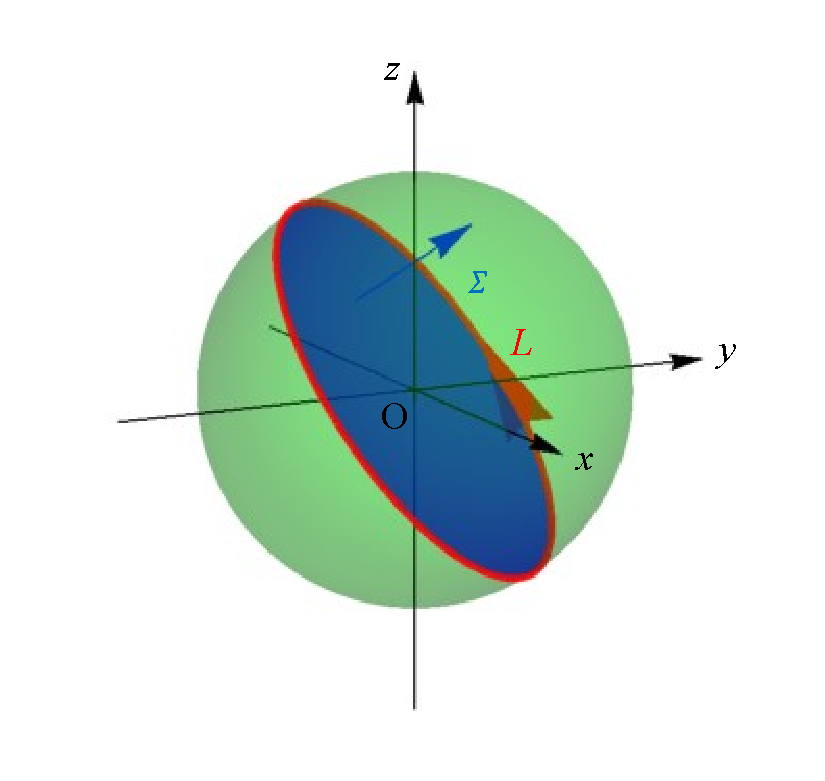
\includegraphics[height=0.5\textheight]{Figures24/Fig13-5-2-1.pdf}
\end{center}
\caption{例9图示}
\label{13-5-2-1}
\end{figure}

解:记$\Sigma$是平面$x+y+z=0$上$L$围成的部分,$\Sigma$与$L$的方向符合右手法则,记$\Sigma$的上侧为正,

$\because y,z,x\in C^1$,

$\therefore\BLOInt L{y\md x+z\md y+x\md z}=\BSIInt\Sigma{\begin{vmatrix}
\bm i&\bm j&\bm k\\
\frac\partial{\partial x}&\frac\partial{\partial y}&\frac\partial{\partial z}\\
y&z&x
\end{vmatrix}\bm\cdot\bm n\md S}=\BSIInt\Sigma{(\pp xy-\pp zz,\pp zy-\pp xx,\pp zx-\pp yy)\bm\cdot\bm n\md S}\\
=\BSIInt\Sigma{(0-1,0-1,0-1)\bm\cdot\bm n\md S}=\BSIInt\Sigma{(-1,-1,-1)\bm\cdot\bm n\md S}$,

$\because\Sigma$的单位法向量为$\bm n=(1,1,1)\frac1{\sqrt3}$,

$\therefore\BLOInt L{y\md x+z\md y+x\md z}=\BSIInt\Sigma{(-1,-1,-1)\bm\cdot(1,1,1)\frac1{\sqrt3}\md S}=\frac1{\sqrt3}\BSIInt\Sigma{-3\md S}=-\sqrt3\pi R^2$.
\item[例10]求电场$\bm v=\frac{\bm r}{r^3}$穿过包围原点的任意简单光滑闭曲面的电通量,其中$r,\bm r$同题5.

\begin{figure}[H]
\begin{center}
\subfigure[]{\label{13-6-9-1}{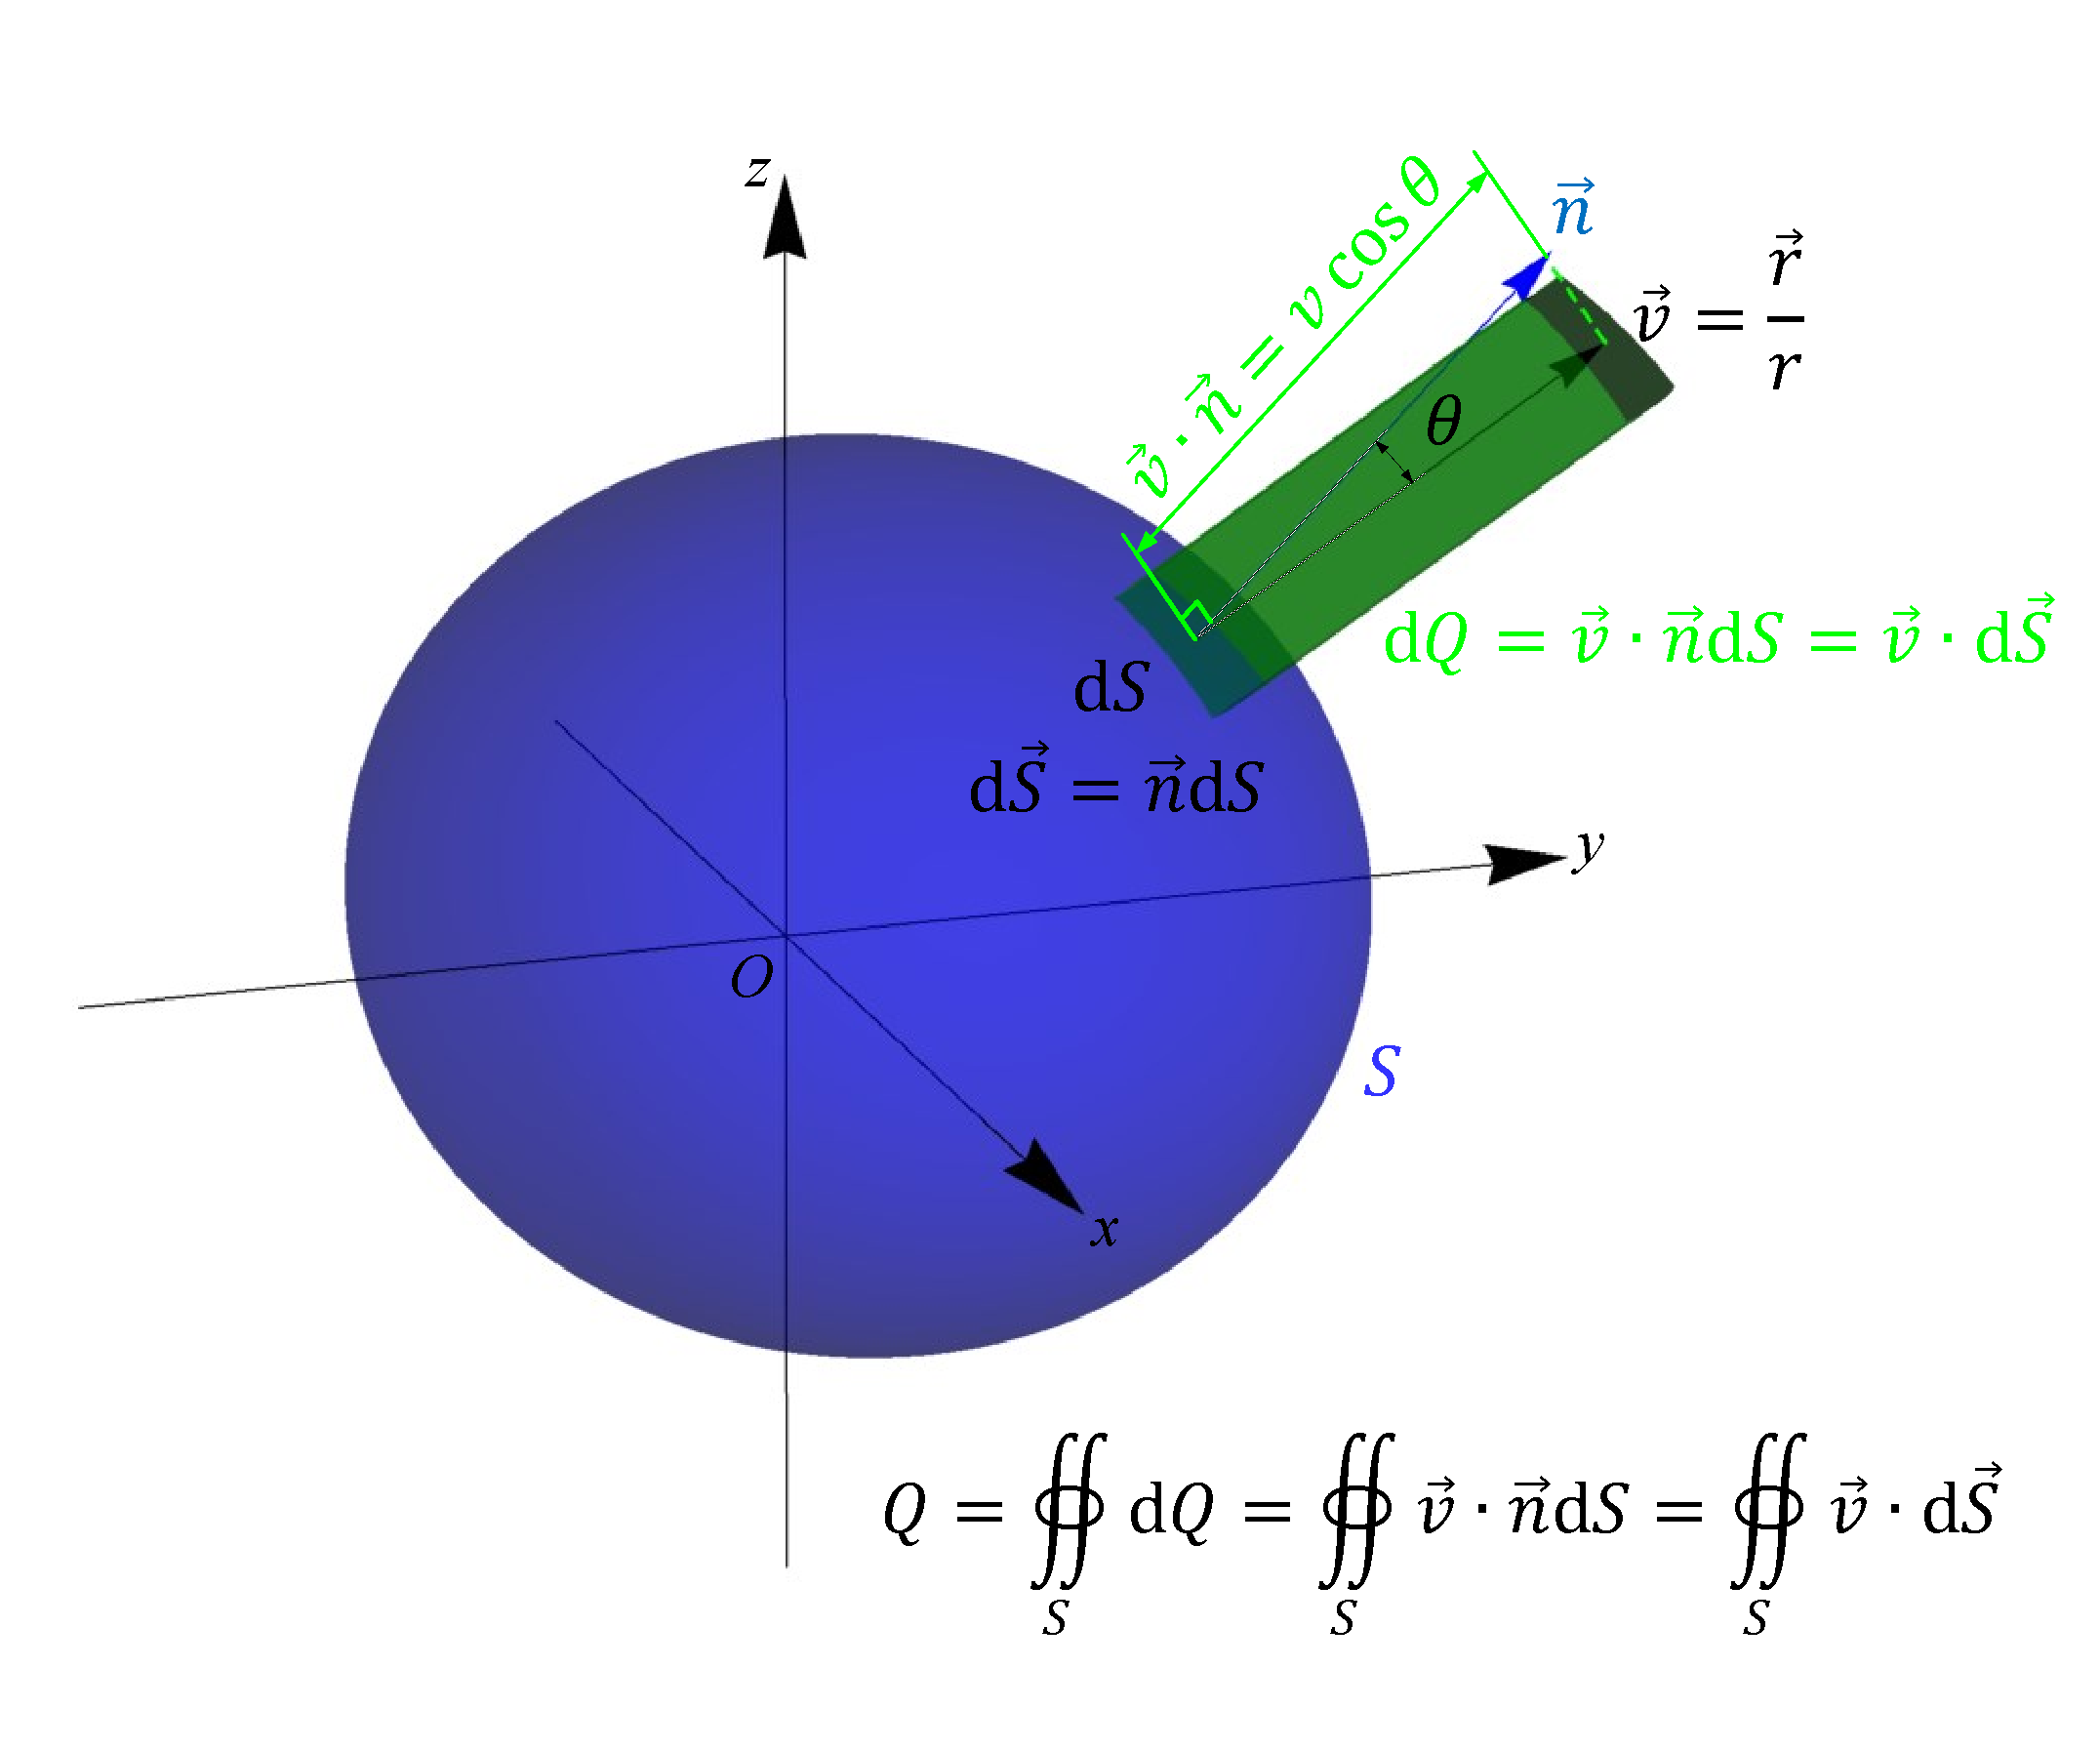
\includegraphics[height=0.58\textheight]{Figures20190613/Fig13-6-9-1.pdf} }}
\end{center}
\end{figure}
\addtocounter{figure}{-1}
\begin{figure}[H]
\addtocounter{figure}{1}
\begin{center}
\subfigure[]{\label{13-6-9-2} {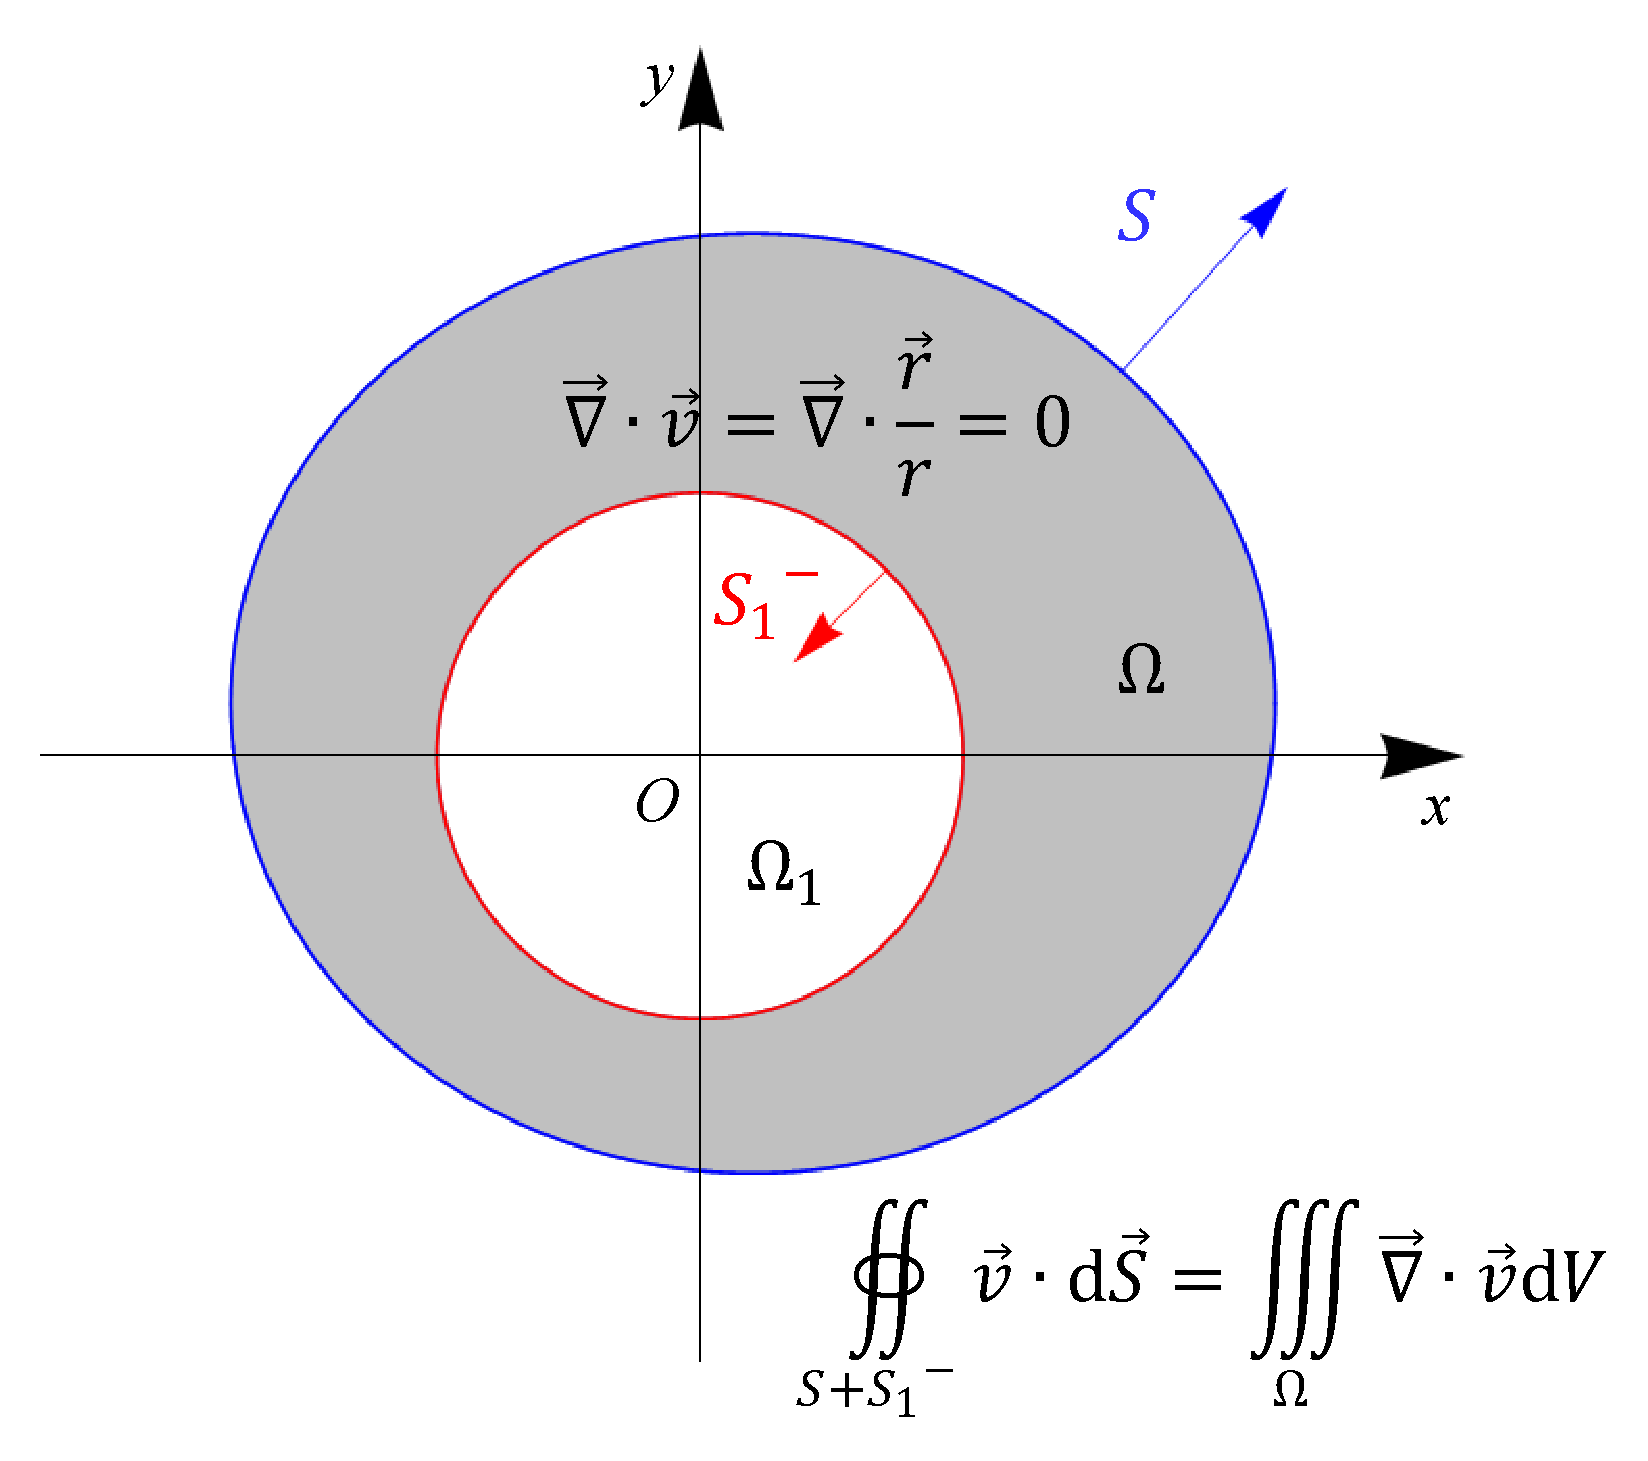
\includegraphics[height=0.6\textheight]{Figures20190613/Fig13-6-9-2.pdf} }}
\end{center}
\caption{例10图示}
\label{13-6-9}
\end{figure}

解:设$S$是包围原点的任意简单光滑闭曲面,$S_1$是$S$围成区域中的包围原点的任意简单光滑闭曲面,$S_1,S$外侧为正,记$S,S_1^-$围成的区域为$\Omega$,

则$\BSOIInt S{\bm v\bm\cdot\md\bm S}-\BSOIInt{S_1}{\bm v\bm\cdot\md\bm S}=\BSOIInt S{\bm v\bm\cdot\md\bm S}+\BSOIInt{S_1^-}{\bm v\bm\cdot\md\bm S}=\BSOIInt{S+S_1^-}{\bm v\bm\cdot\md\bm S}$,

$\because\Omega$不包含原点,

$\therefore\bm v\in C^1(\Omega)$且由上述题8(2)可知$\bm\nabla\bm\cdot\bm v=0$,

$\therefore\BSOIInt{S+S_1^-}{\bm v\bm\cdot\md\bm S}=\IIInt\Omega{\bm\nabla\bm\cdot\bm v}V=\IIInt\Omega0V=0$,

$\therefore\BSOIInt S{\bm v\bm\cdot\md\bm S}=\BSOIInt{S_1}{\bm v\bm\cdot\md\bm S}$,

$\therefore\bm v=\frac{\bm r}{r^3}$穿过包围原点的任意简单光滑闭曲面的电通量都相等,故可取一个特殊的曲面计算电通量的值.

不妨取$S_1:r=a,a>0$,记$\Omega_1$是$S_1$围成的区域,

$\therefore\BSOIInt{S_1}{\bm v\bm\cdot\md\bm S}=\BSOIInt{S_1}{\frac{\bm r}{r^3}\bm\cdot\md\bm S}=\BSOIInt{S_1}{\frac{\bm r}{a^3}\bm\cdot\md\bm S}=\frac1{a^3}\BSOIInt{S_1}{\bm r\bm\cdot\md\bm S}=\frac1{a^3}\IIInt{\Omega_1}{\bm\nabla\bm\cdot\bm r}V\\
=\frac1{a^3}\IIInt{\Omega_1}{(\pp xx+\pp yy+\pp zz)}V=\frac1{a^3}\IIInt{\Omega_1}{3}V=\frac3{a^3}\IIInt{\Omega_1}{}V=\frac3{a^3}\frac43\pi a^3=4\pi$.\footnotemark\footnotetext{该题给出了真空中点电荷电场的高斯定理的证明. 真空中位于原点的点电荷$q$产生的电场
\[\bm E=\frac q{4\pi\varepsilon_0}\frac{\bm r}{r^3}=\frac q{4\pi\varepsilon_0}\bm v,\]

故该电场穿过包围该电荷的任意简单光滑闭曲面的电通量
\[\BSOIInt S{\bm E\bm\cdot\md\bm S}=\frac q{4\pi\varepsilon_0}\BSOIInt S{\bm v\bm\cdot\md\bm S}=\frac q{\varepsilon_0}.\]

即真空中的电荷的电场穿过包围该点电荷的任意简单光滑闭曲面的电通量与该电荷的电量成正比.

}
\end{enumerate}
\end{document}